
This section provides a full description of our proposal called \textit{Variable Space Diversity based MOEA} 
(\VSDMOEA{})~\footnote{The source code in C++ is freely available at \url{https://github.com/joelchaconcastillo/VSD-MOEA.git}}.
%
The novelty of \VSDMOEA{} appears in the replacement phase, which incorporates
the use of variable space diversity and a novel objective space density estimator. 
%
The main principle behind the design of the novel replacement is to use the stopping criterion and 
elapsed generations with the aim of gradually moving from exploration to exploitation during the search process.
%
Note that this principle might be incorporated in any of the three categories of \MOEAS{}.
%
In this paper, our decision was to incorporate it into a dominance-based approach.
%
Note that this category has been particularly suitable for problems with two and three objectives.
%
Thus, some of our design decisions might not be suitable for dealing with many-objective optimization problems.
\begin{algorithm}[h]
%\algsetup{linenosize=\tiny}
	\caption{Main procedure of VSD-MOEA} 
	\begin{small}
\begin{algorithmic}[1]
 	\STATE \textbf{Initialization}: Generate an initial population $P_0$ with $N$ individuals.
	\STATE \textbf{Evaluation}: Evaluate all individuals in the population.
	\STATE Assign $t=0$
	\WHILE{ (not stopping criterion)  }
	   \STATE \textbf{Mating selection}: Fill the mating pool by performing binary tournament selection on $P_t$, 
		 based on the non-dominated ranks (ties are broken randomly).
	   \STATE \textbf{Variation}: Apply SBX and Polynomial-based mutation to the mating pool to create an offspring population $Q_t$
		 with $N$ individuals.
		 \STATE \textbf{Evaluation}: Evaluate all individuals in $Q_t$.
	   \STATE \textbf{Survivor selection}: Generate $P_{t+1}$ by applying the replacement scheme 
		 described in Algorithm~\ref{alg:Replacement_Phase}, using $P_t$ and $Q_t$ as inputs.
	   \STATE $t=t+1$
	\ENDWHILE
	\end{algorithmic}
	\end{small}
\label{alg:vsd-moea}
\end{algorithm}

The general framework of \VSDMOEA{} is quite standard.
%
Algorithm~\ref{alg:vsd-moea} shows the pseudo-code of \VSDMOEA{}.
%
Parents are selected using a binary tournament based on dominance ranking with ties broken randomly.
%
The variation stage is based on applying the well-known Simulated Binary Crossover (SBX) 
and polynomial-based mutation~\citep{Joel:SBX1994, Joel:Mutation} operators.
%
Thus, the contribution appears in the replacement phase.
%
The rest of this section is devoted to describing the replacement phase, including the novel objective space density 
estimator.

\subsection{Replacement Phase of VSD-MOEA}

The replacement phase of \EAS{} is in charge of deciding, for each generation, which members of the previous population together with their corresponding offspring will survive.
%
The novel replacement scheme promotes a gradual movement from exploration to exploitation, which has been a highly 
beneficial principle in the design of single-objective optimizers~\citep{Joel:MULTI_DYNAMIC}.
%
Specifically, the replacement phase operates as follows.
%
First, the members of the previous population and offspring are merged in a multi-set with $2 \times N$ individuals.
%
Then, an iterative process that selects an additional
individual at each iteration is used to pick the $N$ survivors. 
%
In order to take into account the diversity of decision variable space, the Distance to Closest Survivor (\DCS{}) of each
individual is calculated at each iteration.
%
Thus, the \DCS{} of an individual $I$ is calculated as $\displaystyle{\min_{s \in S}\ Distance(I, s)}$,
where $S$ is the multi-set containing the currently selected survivors. 
%
Normalized Euclidean distances are considered, so in order to calculate distances between any two individuals $A$ and $B$, 
Eq.~(\ref{eqn:distance}) is applied.
%
In the first iteration, the $S$ multi-set is empty, so the \DCS{} of each individual is infinity.
%
\begin{equation}\label{eqn:distance}
Distance(A, B) =   \left ( \frac{1}{n}  \sum_{i=1}^n \left ( \frac{A_i - B_i}{x_i^{(U)} - x_i^{(L)}} \right )^2  \right)^{1/2}
\end{equation}

Note that individuals with larger \DCS{} values are those that contribute more significantly to promoting exploration.
%
In order to avoid an excessive decrease in the degree of exploration, individuals with a \DCS{} value below a certain threshold are penalized.
%
Then, among the non-penalized individuals, an objective space density estimator is used to select the additional
survivor of the iteration.
%
In our case, the novel density estimator described in the next subsection is used. 
%
Note that it might happen that all individuals are penalized, in which case the individual with the largest \DCS{} is selected to survive.


In order to better understand the penalty method, it can be visualized in the following way.
%
After selecting each survivor, a hyper-sphere 
centered around a candidate solution --- in decision variable space --- is created.
%
Then, all the individuals that are inside the hyper-sphere are penalized, with the objective space density estimator only taking 
into account the survivors and the non-penalized individuals.
%
This is illustrated in Fig.~\ref{fig:Hypersphere} (below), which represents a state where three individuals have been 
selected to survive and an additional survivor must be picked.
%
The left side shows individuals in decision variable space.
%
Current survivors are marked with a red border. Each of them is surrounded by a dashed blue circle of 
radius $D_t$.
%
In this scenario, the penalized individuals are numbers 4, 5, and 6.
%
In objective function space --- right side --- the penalized individuals are shown in gray, indicating
that the objective space density estimator is not considering them.
\begin{figure}[h]
\centering
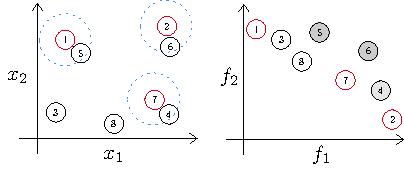
\includegraphics[width=0.5\textwidth]{Images/Diagram.pdf}
\caption{Penalty Method of the Replacement Phase - The left side represents decision variable space and the right side represents 
objective function space.} \label{fig:Hypersphere}
\end{figure}

Since using a large radius for the hyper-spheres induces a large degree of 
exploration, it makes sense to reduce this value during the optimization process.
%
This is precisely one of the keys of our proposal.
%
The sizes of the hyper-spheres are modified dynamically by taking into account the stopping 
criterion and elapsed generations.
%
Specifically, the radius is decreased linearly starting from an initial distance.
%
This means that in the initial phases, exploration is promoted.
%
However, as the size of the radius decreases, only very close individuals are penalized, meaning that more 
exploitation is allowed.
%
Note that this method requires a parameter that is the initial radius of the 
hyper-spheres or initial threshold value.
%
This parameter is denoted by $D_I$. 
%
Assigning a large value to this parameter might result in many individuals being penalized, which might thus maintain non-useful diversity.
%
However, a value that is too small might not prevent fast convergence, meaning the approach  
might behave as a traditional non-diversity based \MOEA{}.
%
The robustness of the proposal with respect to this additional parameter is studied in our experimental validation.

\begin{algorithm}[h]
\algsetup{linenosize=\tiny}
	\caption{Replacement Phase of VSD-MOEA} 
\begin{small}
\begin{algorithmic}[1]
\STATE Input: $P_t$ (Population of current generation), $Q_t$ (Offspring of current Generation)
    	\STATE Output: $P_{t+1}$ 
        \STATE $R_t = P_t \cup Q_t$ \label{alg:1}
        \STATE $P_{t+1} = \emptyset$ \label{alg:2}
        \STATE $Penalized = \emptyset$ \label{alg:3}
				\STATE $D_t = D_I - D_I * \frac{G_{Elapsed}}{0.5*G_{End}}$ \label{alg:4}
        \WHILE{ $|P_{t+1}|$ $\leq$ N } \label{alg:6}
					\STATE Compute $DCS$ of individuals in $R_t$, using $P_{t+1}$ as a reference set \label{alg:7}
					\STATE Move the individuals in $R_t$ with $DCS < D_t$ to $Penalized$ \label{alg:8}
        	\IF{$R_t$ is empty} \label{alg:9}
						\STATE Compute $DCS$ of individuals in $Penalized$, using $P_{t+1}$ as a reference set \label{alg:10}
						\STATE Move the individual in $Penalized$ with the largest $DCS$ to $R_t$ \label{alg:11}
        	\ENDIF
					\STATE Identify the first front ($F$) in $R_t \cup P_{t+1}$ with an individual $I \in R_t$ \label{alg:12}
					\STATE Use the novel density estimator (Algorithm~\ref{alg:Density_Estimator}) to select a new survivor 
					from $F$ and move it to $P_{t+1}$\label{alg:13}
        \ENDWHILE
    	\RETURN $P_{t+1}$ \label{alg:14}
	\end{algorithmic}
\end{small}
\label{alg:Replacement_Phase}
\end{algorithm}

Algorithm~\ref{alg:Replacement_Phase} formalizes the replacement phase of \VSDMOEA{}.
%
First, the population of the previous generation ($P_t$) and the offspring ($Q_t$) are merged
in $R_t$ (line \ref{alg:1}).
%
At each iteration, the multi-set $R_t$ contains the remaining non-penalized individuals that might be selected 
to survive.
%
The population of survivors ($P_{t+1}$) and the set containing the penalized individuals are initialized to
the empty set (lines \ref{alg:2} and \ref{alg:3}).
%
Then, the threshold value ($D_t$) that is used to penalize individuals that are too close is calculated (line \ref{alg:4}).
%
Note that $D_I$ denotes the initial threshold value, $G_{Elapsed}$ is the number of generations that have 
evolved, and $G_{End}$ is the stopping criterion, i.e., the number of generations that are to be evolved 
during the execution of the \VSDMOEA{}.
%
The linear decrease is calculated such that after $50\%$ of the total number of 
generations, the $D_t$ value is below 0, meaning that no penalties are applied.
%
This means that in the first $50\%$ of the generations, more exploration is induced than in traditional MOEAs.
%

Then, an iterative process that selects an individual in each iteration is executed until the survivor
set contains $N$ individuals (line \ref{alg:6}).
%
The iterative process works as follows.
%
First, the \DCS{} value of each remaining non-penalized individual is calculated (line \ref{alg:7}).
%
Then, those individuals with a \DCS{} value lower than $D_t$ are moved to the set of penalized individuals (line \ref{alg:8}).
%
If all the remaining individuals are penalized (line \ref{alg:9}), it means that the amount of exploration is lower than desired.
%
Thus, the individual with the largest \DCS{} value is recovered, i.e., moved to the set of non-penalized individuals (lines \ref{alg:10} and \ref{alg:11}), and thus survives.
%
Finally, the objective function space is considered.
%
Specifically, candidate non-penalized individuals and current survivors are merged.
%
Then, the well-known non-dominated sorting procedure proposed in ~\cite{Joel:NSGAII} is executed on this set, stopping as soon as a front with 
a candidate individual is found, i.e. with an individual of $R_t$ (line \ref{alg:12}).
%
Then, taking the identified front as an input, a novel objective space density estimator is used to select
the next survivor (line \ref{alg:13}).
%
The specific way in which each individual's contribution to the diversity of the objective space is measured is described in the next section.
%

\subsection{A Novel Density Estimator for Objective Function Space}
\label{subsection:density}


Since the dominance definition is not related to the preservation of diversity in objective function space,
dominance-based \MOEAS{} usually incorporate objective-space density estimators to promote the survival
of diverse individuals.
%
As previously described, our density estimator selects a new survivor from the front identified
in line \ref{alg:13} of Algorithm~\ref{alg:Replacement_Phase}.
%
This front (referred in Algorithm~\ref{alg:Density_Estimator} as $F$) contains at least one 
individual belonging to $R_t$, and it might also contain some elements 
of $P_{t+1}$.
%
The aim behind the selection of the next survivor is to pick an individual of the input front
that contributes significantly in terms of the quality and diversity of the objective space. % to $R_t$.
\begin{algorithm}[]
\algsetup{linenosize=\tiny}
	\caption{Density estimator} 
\begin{small}
\begin{algorithmic}[1]
\STATE Input: $P_{t+1}$ (Survivors), $R_t$ (Candidates), $F$ (Current front)
    	\STATE Output: $I \in R_t$ 
	\STATE $FP = P_{t+1} \cap F$ \label{alg:FP}
	\STATE $FR = R_{t} \cap F$ \label{alg:FR}
        \FOR{$k \in$ number of objectives}\label{alg:density_for}
	      \STATE Select the best individual $I \in F$ of $k$ according to Eq.~\ref{eqn:extremes}.\label{alg:density_1}
	  	\IF{ $I \in FR$}
	  	 \RETURN $I$ \label{alg:density_2}
	  	\ENDIF
	\ENDFOR\label{alg:density_endfor}
	\STATE $MaxID = 0$ \label{alg:density_for2}
	\FOR{ $ Ic \in FR$}
	\STATE $Improvement = \displaystyle{\min_{s \in FP}\ ID(Ic, s)}$ 
	\IF{ $Improvement > MaxID$} \label{alg:density_if2}
	   \STATE $MaxID = Improvement$
	   \STATE $I = Ic$ 
	\ENDIF \label{alg:density_endif2}
	\ENDFOR	\label{alg:density_endfor2}
    	\RETURN $I$ \label{alg:density_4}
	\end{algorithmic}
\end{small}
\label{alg:Density_Estimator}
\end{algorithm}

Algorithm~\ref{alg:Density_Estimator} describes the selection of the next survivor.
%
First, the sets $FP$ and $FR$ are identified (lines \ref{alg:FP} and \ref{alg:FR}).
%
$FP$ contains the current survivors that are in $F$ (already selected to the next generation $P_{t+1}$), whereas $FR$ contains
the remaining non-penalized individuals that are in $F$.
%
Then, similarly to most state-of-the-art algorithms, a step to promote the selection of boundary solutions
is included.
%
Note that selecting the best solution for each objective might cause some drawbacks related to accepting a small improvement
in one objective at the expense of significant degradation in other objectives, this issue can be resolved 
by applying augmented functions, which is the alternative used by~\cite{deb2016optimality}.
%
Specifically, for each objective $k$, the candidate solution that minimizes the Augmented Function (AF)
given in Eq.~\ref{eqn:extremes} is iteratively identified (lines \ref{alg:density_for} to \ref{alg:density_endfor}).
%
If this individual belongs to $FR$, i.e., it has not yet been selected as a survivor, the next survivor is such an individual
and the process ends (line \ref{alg:density_2}).
%
Note that augmented functions usually take into account weight vectors in order to deal with objectives
that exhibit very different scales.
%
Since benchmarks that have similar scales in each objective have been used in this paper, there was no need to apply
the aforementioned weight vectors.

\begin{equation}\label{eqn:extremes}
AF_k (\vec{x}) = f_k(\vec{x}) + 10^{-4} \times  \sum_{j=1}^M f_j( \vec{x} )
\end{equation}

In cases where the individuals that optimize each $AF_K$ function are already in $P_{t+1}$, a contribution
to objective-space diversity is calculated for each individual in $FR$ (lines \ref{alg:density_for2} to \ref{alg:density_4}).
%
This contribution is calculated by taking into account the current survivors of the front ($FP$).
%
Specifically, the ``Improvement Distance'' ($ID$) defined for the indicator IGD+~\citep{Joel:Inverted_Generational_Distance_Plus}
is used.
%
The $ID$ of an individual $A$ with respect to an individual $B$ is calculated by taking into account only the objectives
where $A$ is better.
%
Specifically, Eq.~(\ref{eq:ImprovementDistance}) is used.

\begin{equation} \label{eq:ImprovementDistance}
\begin{split}
 ID(A, B) = &  \left (\sum_{i=1}^M \left (max(0, f_i(B) - f_i(A) \right ))^2  \right)^{1/2}
\end{split}
\end{equation}

The contribution of each member in $FR$ $(I)$ is calculated as $\displaystyle{\min_{s \in FP}\ ID(I, s)}$.
%
Then, the individual with the highest contribution is selected as the next survivor (lines \ref{alg:density_if2} 
to \ref{alg:density_endif2}).

